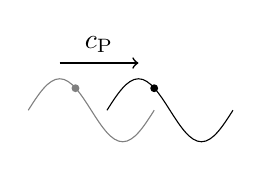
\begin{tikzpicture}[scale=2]
\draw[gray] ( 0.0, 0) sin ( 0.2, 0.2) cos ( 0.4, 0) sin ( 0.6,-0.2) cos ( 0.8, 0);
\fill[gray] (0.3, 0.14) circle[radius=0.025];
\draw ( 0.5, 0) sin ( 0.7, 0.2) cos ( 0.9, 0) sin ( 1.1,-0.2) cos ( 1.3, 0);
\fill (0.8, 0.14) circle[radius=0.025];
\draw[->, semithick] ( 0.2, 0.3) -- node[above] {$c_\mathrm{P}$} (0.7, 0.3);
\end{tikzpicture}
